\documentclass[aspectratio=169,11pt]{beamer}
\usetheme[progressbar=frametitle,numbering=fraction]{metropolis}
\setbeamerfont{normal text}{size=\small}
\metroset{sectionpage=none}
\AtBeginDocument{\usebeamerfont{normal text}}
\usepackage[utf8]{inputenc}
\usepackage[T1]{fontenc}
\usepackage[spanish,es-noshorthands,es-nodecimaldot]{babel}
\usepackage{booktabs}
\usepackage{amsmath,amssymb}
\usepackage{tikz}
\usetikzlibrary{positioning,arrows.meta}
\usepackage{qrcode}

% Colores UNI (granate)
\definecolor{uni}{HTML}{8B1E2D}
\definecolor{unidark}{HTML}{3B0D14}
\definecolor{ok}{HTML}{0F766E}
\definecolor{bad}{HTML}{B91C1C}
\definecolor{azul}{HTML}{1F4E9A}
\definecolor{azuldark}{HTML}{0B2545}
\setbeamercolor{frametitle}{bg=azuldark,fg=white}
\setbeamercolor{progress bar}{fg=azul,bg=azul!20}
\setbeamercolor{title separator}{fg=azul}
\setbeamercolor{background canvas}{bg=white}
\setbeamercolor{standout}{bg=azuldark,fg=white}
\setbeamercolor{title}{fg=azuldark}
\setbeamercolor{alerted text}{fg=uni}
\setbeamercolor{example text}{fg=ok}
\setbeamertemplate{caption}{\insertcaption}

% Expositor sugerido (esquina inferior izquierda)
\newcommand{\expositor}[1]{%
  \begin{tikzpicture}[remember picture,overlay]
    \node[anchor=south west,font=\scriptsize\color{gray},xshift=4mm,yshift=1.5mm] at (current page.south west) {#1};
  \end{tikzpicture}}
\newcommand{\num}[1]{\textbf{\color{uni}#1}}
\tikzset{box/.style={draw, rounded corners=2pt, align=center, minimum height=10mm, inner sep=3pt, fill=#1}, box/.default=white}

\title[Diagnóstico de fallas en rodamientos]{Diagnóstico de fallas en rodamientos\\con pocos datos de falla y cambio de carga}
\subtitle{CNN, Audio Spectrogram Transformer y aumento por difusión condicional}
\author{\textbf{Grupo 6}\\Hipólito Eusebio Coaguila Berrios · Lenin Dixon Herrera Padilla · Jhafet Martín Cánepa Maceda}
\institute{MIA-203 Redes Neuronales y Aprendizaje Profundo · Maestría en Inteligencia Artificial · FIIS -- UNI\\Docente: Aldo Camargo Fernández-Baca, Ph.D.}
\date{6 de noviembre de 2026}
\titlegraphic{\begin{tikzpicture}[remember picture,overlay]
  % marco doble azul
  \draw[azuldark,line width=2.2pt,rounded corners=6pt]
    ([xshift=3mm,yshift=3mm]current page.south west) rectangle ([xshift=-3mm,yshift=-3mm]current page.north east);
  \draw[azul,line width=0.6pt,rounded corners=4pt]
    ([xshift=4.6mm,yshift=4.6mm]current page.south west) rectangle ([xshift=-4.6mm,yshift=-4.6mm]current page.north east);
  % franja inferior
  \fill[azuldark,rounded corners=4pt] ([xshift=4.6mm,yshift=4.6mm]current page.south west) rectangle ([xshift=-4.6mm,yshift=10mm]current page.south east);
  \node[anchor=west,font=\scriptsize\color{white},xshift=9mm,yshift=7.3mm] at (current page.south west) {Universidad Nacional de Ingeniería · Lima, Perú};
  \node[anchor=east,font=\scriptsize\color{white},xshift=-9mm,yshift=7.3mm] at (current page.south east) {Examen final · MIA-203};
  % logo
  \node[anchor=north east,xshift=-8mm,yshift=-7mm] at (current page.north east) {
\includegraphics[height=2.2cm]{figs/logo_uni.png}};
\end{tikzpicture}}

\begin{document}

\maketitle

% =====================================================================
\section{Problema y motivación}

\begin{frame}{¿Por qué importa?}
\begin{columns}[T]
\column{0.55\textwidth}
\begin{itemize}
\item Los rodamientos causan el \num{41--44\,\%} de las fallas de los motores eléctricos (encuestas IEEE y EPRI).
\item Una falla sin aviso detiene la máquina y la línea de producción.
\item \alert{Mantenimiento predictivo}: un acelerómetro barato y un modelo que avisa \emph{antes} de la parada.
\end{itemize}
\vspace{2mm}
\textbf{En el Perú:} molinos, fajas y bombas de la minería; bombas de riego y cámaras de frío de la agroindustria; bombeo de agua.
\column{0.42\textwidth}
\centering
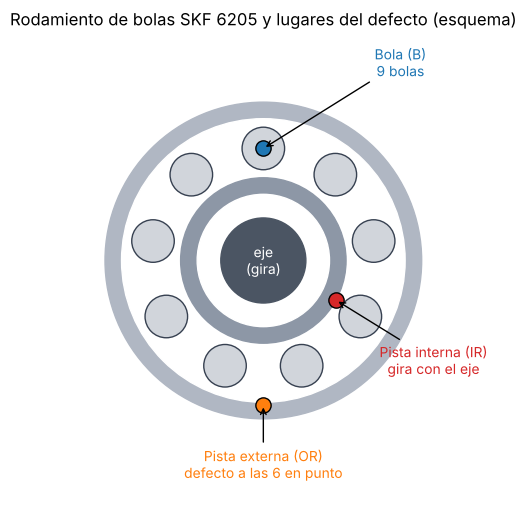
\includegraphics[width=0.72\linewidth]{figs/rodamiento.png}\\
{\scriptsize Rodamiento SKF 6205 y lugares del defecto}
\end{columns}
\end{frame}

\begin{frame}{Formulación del problema}
\begin{columns}[T]
\column{0.5\textwidth}
\begin{block}{Entrada y salida}
\textbf{Entrada:} ventana de vibración $x\in\mathbb{R}^{2048}$ (171~ms a 12~kHz)\\[1mm]
\textbf{Salida:} una de \num{10} clases: Normal o falla en bola / pista interna / pista externa, con 3 severidades
\end{block}
\begin{block}{Éxito}
F1-macro en una \alert{carga del motor nunca vista} (3~HP), recall de las fallas escasas y robustez al ruido.
\end{block}
\column{0.47\textwidth}
\begin{alertblock}{Dos dificultades reales de planta}
\begin{enumerate}
\item \textbf{Pocos datos de falla}: las graves son rarísimas\\ $\Rightarrow$ desbalance inducido 30\,\% / 10\,\% / \num{3\,\%}
\item \textbf{Cambio de condición}: la máquina opera con cargas no vistas\\ $\Rightarrow$ entrenar 0--2~HP, probar 3~HP
\end{enumerate}
\end{alertblock}
\end{columns}
\end{frame}

% =====================================================================
\section{Trabajos relacionados}

\begin{frame}{Trabajos relacionados}
\scriptsize
\renewcommand{\arraystretch}{1.15}
\begin{tabular}{p{0.27\textwidth}p{0.33\textwidth}p{0.32\textwidth}}
\toprule
Tema & Qué hacen & Nuestra diferencia \\ \midrule
Diagnóstico clásico y CWRU \newline {\scriptsize Randall y Antoni 2011; Smith y Randall 2015} & Envolvente en BPFO/BPFI; CWRU tiene condiciones difíciles & Usamos la física para \emph{verificar} a la red \\
Revisiones DL en CWRU \newline {\scriptsize Neupane y Seok 2020; Zhao et al. 2020} & Exactitudes $\approx$100\,\%, a menudo con fuga & Partición por carga y en el tiempo \\
CNN 1D: WDCNN \newline {\scriptsize Zhang et al. 2017} & CNN sobre la señal cruda & Nuestra línea base \\
Transformer, ViT, AST \newline {\scriptsize Vaswani 2017; Gong 2021} & Atención sobre parches del espectrograma & ¿Se transfiere el audio a vibración? \\
Difusión para desbalance \newline {\scriptsize Ho 2020; Yang 2024; Wang 2024} & Imágenes tiempo-frecuencia, misma condición & Señal 1D, carga no vista, control de sobremuestreo \\
\bottomrule
\end{tabular}
\end{frame}

% =====================================================================
\section{Datos y metodología}

\begin{frame}{Datos: CWRU Bearing Data Center}
\begin{columns}[T]
\column{0.5\textwidth}
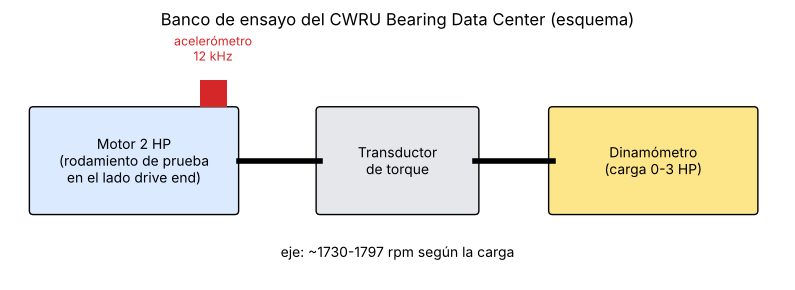
\includegraphics[width=0.72\linewidth]{figs/banco.png}
\small
\begin{itemize}
\item Motor de 2~HP, acelerómetro \emph{drive end}, 12~kHz
\item 4 cargas (0--3~HP, 1797--1730~rpm)
\item \num{40} archivos = 10 clases $\times$ 4 cargas, $\sim$10~s c/u
\end{itemize}
\column{0.48\textwidth}
\begin{alertblock}{Dos errores del conjunto, corregidos}
\begin{enumerate}
\item La clase \textbf{Normal está a 48~kHz}, no a 12~kHz: sin corregir, la red podía reconocerla por la escala espectral (atajo).
\item \texttt{99\_Normal\_2.mat} traía una \textbf{copia de la carga 1}.
\end{enumerate}
\end{alertblock}
\centering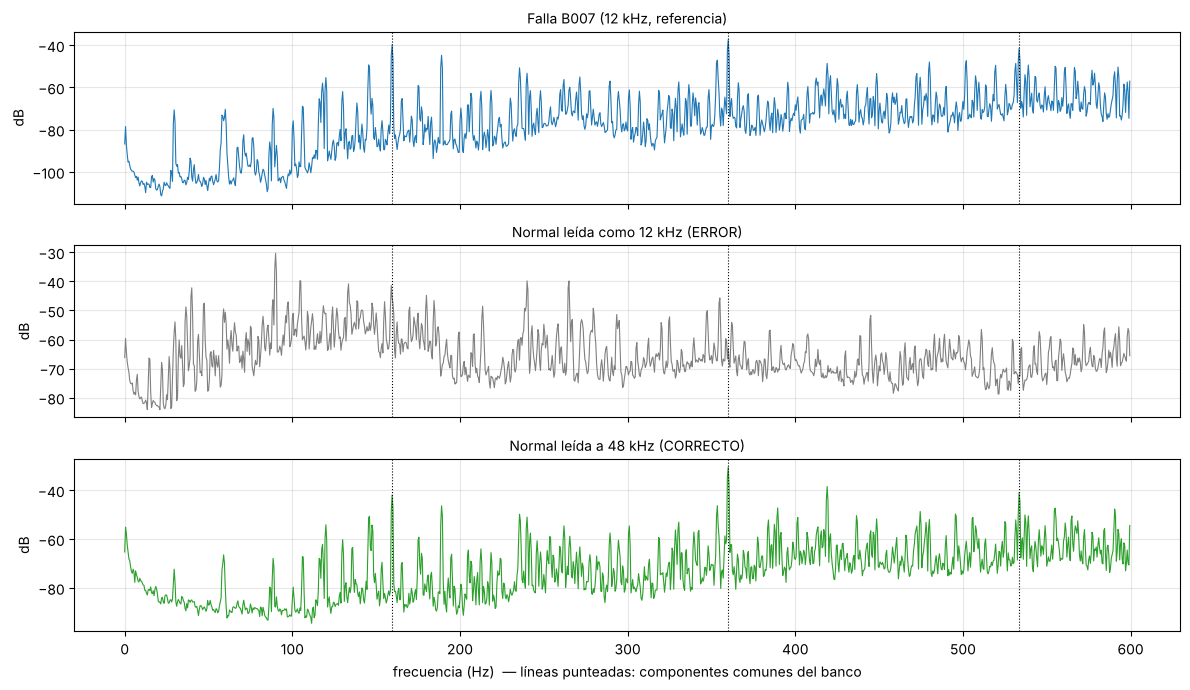
\includegraphics[width=0.5\linewidth]{figs/normal48k.png}
\end{columns}
\end{frame}

\begin{frame}{La física de la falla}
\begin{columns}[T]
\column{0.52\textwidth}
\centering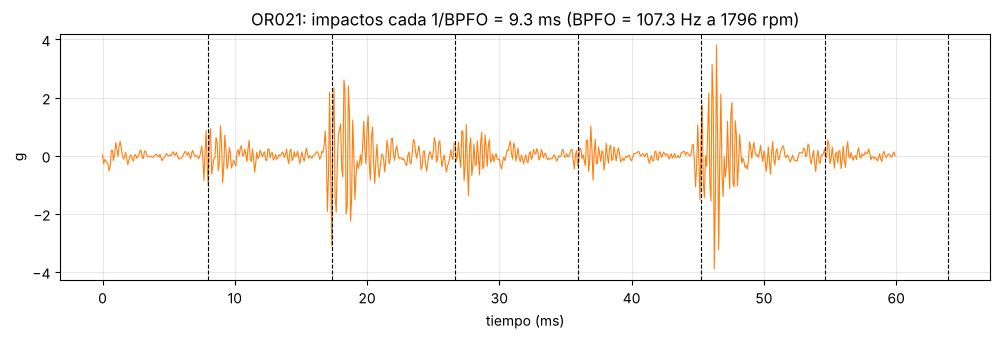
\includegraphics[width=0.85\linewidth]{figs/impactos.png}\\
\raggedright
\small Cada vez que una bola pasa por el defecto hay un \textbf{impacto}. El ritmo depende de dónde está el daño:
\[
\mathrm{BPFO}=\tfrac{N_b}{2}f_r\!\left(1-\tfrac{d}{D}\cos\phi\right)=3{,}585\,f_r
\]
\[
\mathrm{BPFI}=\tfrac{N_b}{2}f_r\!\left(1+\tfrac{d}{D}\cos\phi\right)=5{,}415\,f_r
\]
\column{0.46\textwidth}
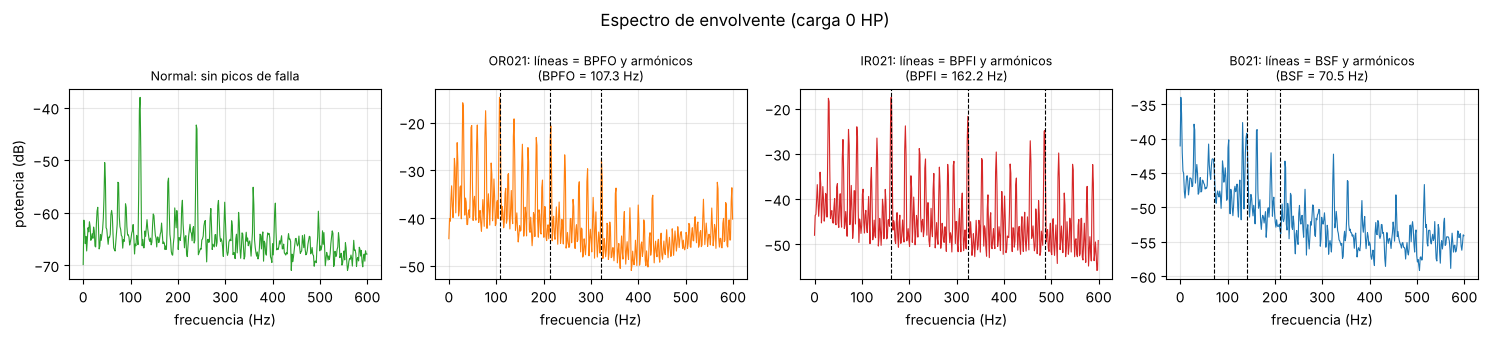
\includegraphics[width=0.95\linewidth]{figs/envolvente.png}
\small Espectro de envolvente: picos en BPFO / BPFI y armónicos. La \alert{bola} es la más difícil (pico débil).\\[1mm]
A 3~HP: BPFO $\approx$ 103~Hz, BPFI $\approx$ 156~Hz.
\end{columns}
\end{frame}

\begin{frame}{Partición sin fuga y desbalance}
\centering
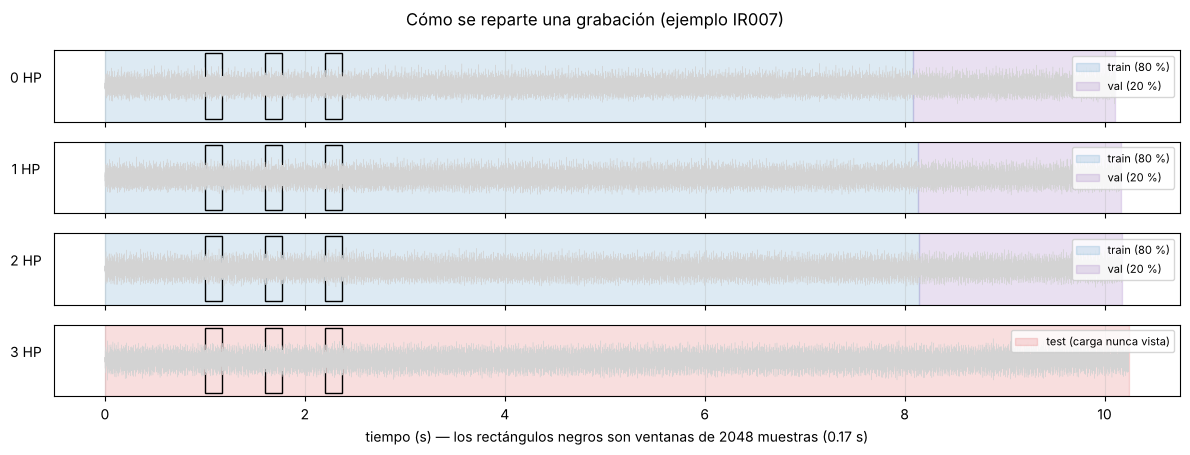
\includegraphics[width=0.58\textwidth]{figs/particion.png}\\[1mm]
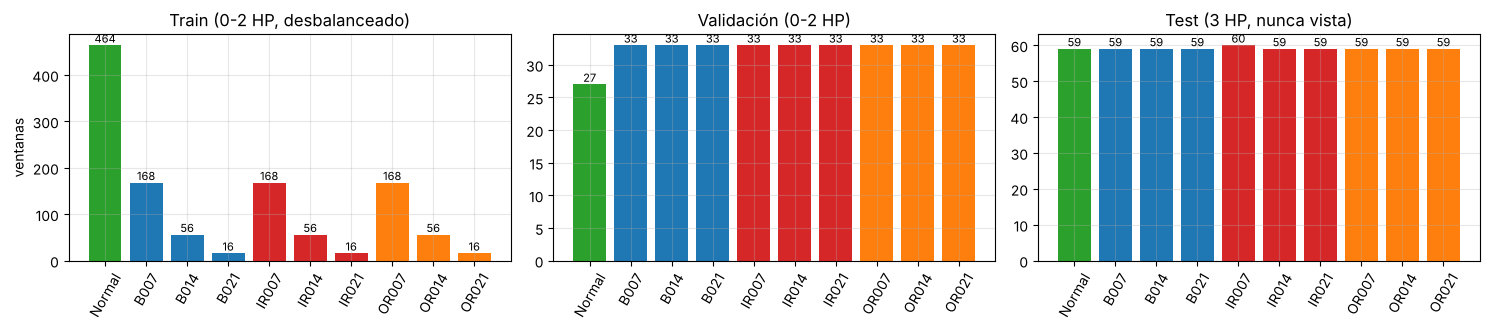
\includegraphics[width=0.75\textwidth]{figs/desbalance.png}\\
\small Train: 1184 ventanas (0--2~HP, 80\,\% inicial) · Val: 324 (20\,\% final, sin solape) · Test: 591 (3~HP completa, \alert{nunca vista})
\end{frame}

\begin{frame}{De la señal a la entrada de cada red}
\centering
\vspace*{-3mm}
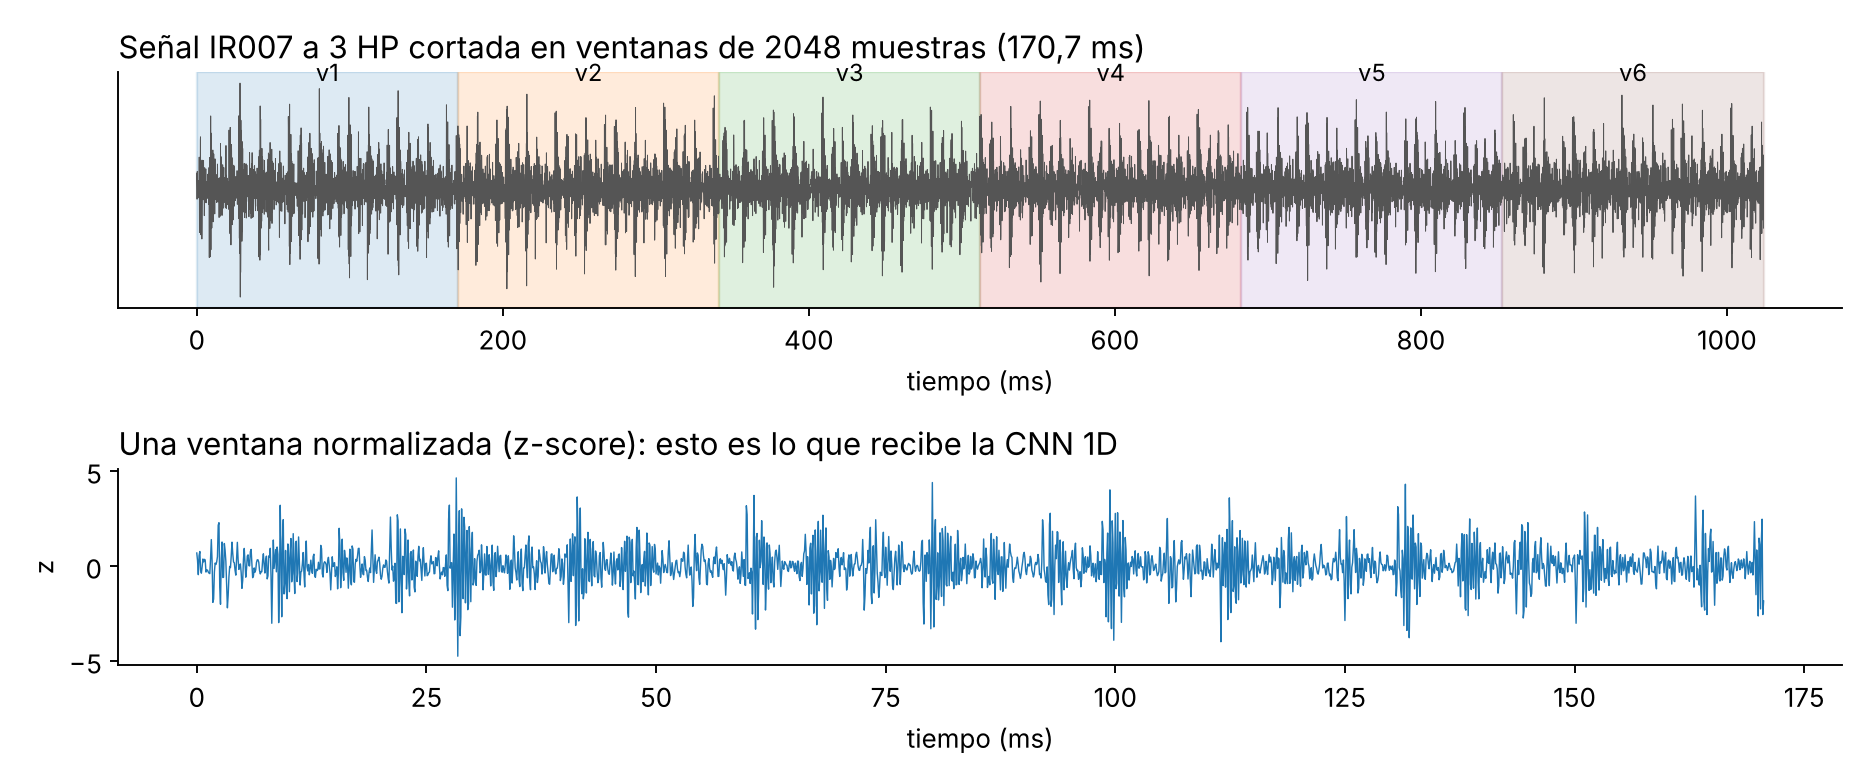
\includegraphics[height=0.33\textheight]{figs/data_ventanas.png}\\[-0.5mm]
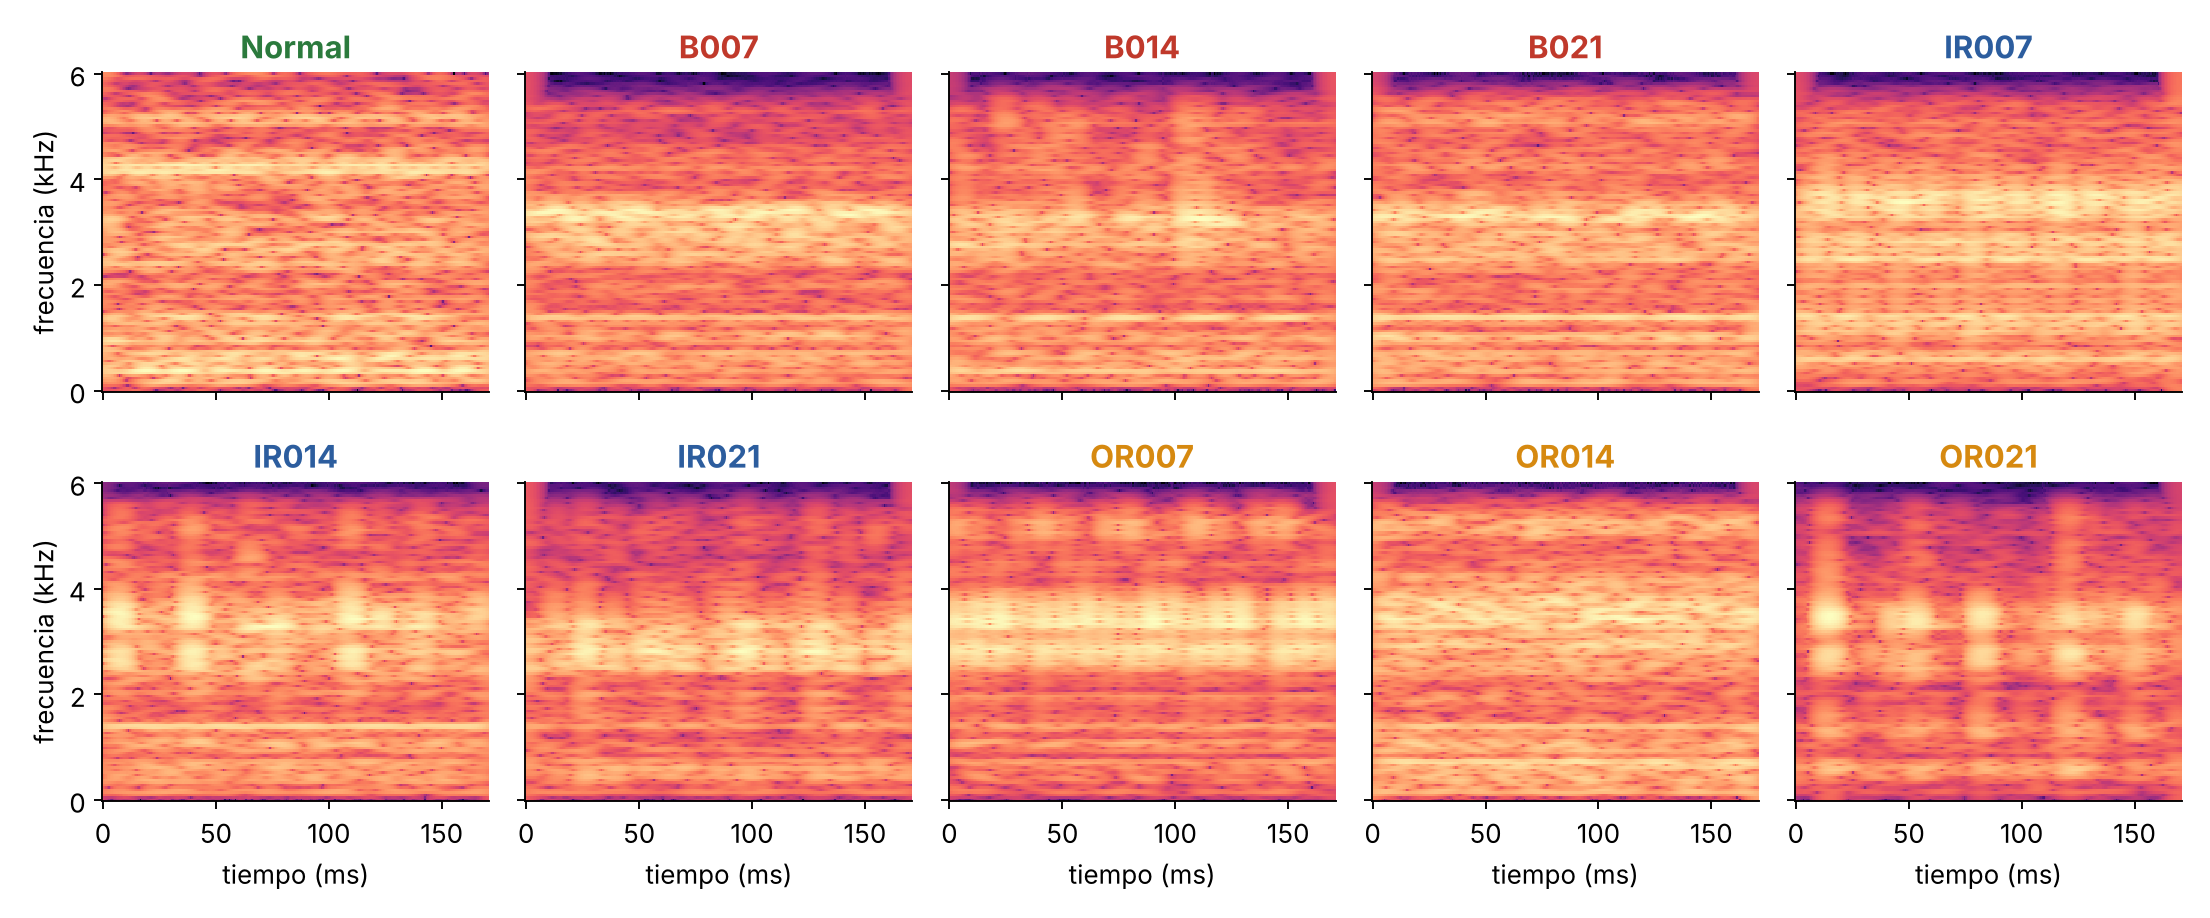
\includegraphics[height=0.37\textheight]{figs/data_espectrogramas.png}\\[-1mm]
\footnotesize Arriba: ventanas para la CNN 1D. Abajo: log-STFT de una ventana por clase (entrada de la CNN 2D); los impactos son \alert{bandas verticales} en 2--4~kHz.
\end{frame}

\begin{frame}{Arquitectura propuesta}
\centering
\resizebox{\textwidth}{!}{%
\begin{tikzpicture}[node distance=3mm and 5mm, font=\small, >={Stealth[length=2mm]}]
\node[box=gray!10] (x) {Ventana $x$\\$1\times2048$};
\node[box=orange!20, below=8mm of x] (ddpm) {\textbf{DDPM 1D condicional}\\U-Net + FiLM($t$, clase)\\guía sin clasificador};
\node[box=gray!10, right=10mm of x] (aug) {Aumento:\\ninguno · sobremuestreo\\clásico · \textbf{difusión}};
\node[box=blue!10, right=10mm of aug, yshift=14mm] (c1) {\textbf{CNN 1D} (WDCNN, 0,04~M): conv k64 s16 $\to$ 4 bloques $\to$ GAP $\to$ 10};
\node[box=blue!10, below=3mm of c1] (c2) {STFT $129{\times}257$ $\to$ \textbf{CNN 2D} (0,24~M) $\to$ GAP $\to$ 10};
\node[box=blue!10, below=3mm of c2] (c3) {16~kHz $\to$ mel $128{\times}96$ $\to$ \textbf{AST} preentrenado (85~M) $\to$ 10};
\node[box=green!15, right=6mm of c2] (y) {$\hat y$\\10 clases};
\draw[->] (x) -- (aug); \draw[->] (x) -- (ddpm); \draw[->] (ddpm.east) -| (aug.south);
\draw[->] (aug.east) -- (c1.west); \draw[->] (aug.east) -- (c2.west); \draw[->] (aug.east) -- (c3.west);
\draw[->] (c1.east) -| (y.north); \draw[->] (c2) -- (y); \draw[->] (c3.east) -| (y.south);
\end{tikzpicture}}
\vspace{2mm}
\begin{columns}[T]
\column{0.5\textwidth}\small
\textbf{CNN 1D vs CNN 2D:} efecto de la representación (señal vs espectrograma).\\
\textbf{CNN 2D vs AST:} efecto del Transformer con preentrenamiento.
\column{0.48\textwidth}\small
\textbf{AST:} remuestreo a 16~kHz (frecuencia de preentrenamiento) y espectrograma en fp32 (evita desbordamiento en fp16).
\end{columns}
\end{frame}



\begin{frame}{Formulación y función de pérdida}
\begin{columns}[T]
\column{0.5\textwidth}
\textbf{Clasificadores} (entropía cruzada):
\[
\mathcal{L}(\theta)=-\frac{1}{N}\sum_{i=1}^{N}\sum_{c=1}^{C} y_{i,c}\log p_\theta(c\mid x_i)
\]
\textbf{DDPM} (predice el ruido):
\[
\mathcal{L}_{\mathrm{DDPM}}=\mathbb{E}\left\|\epsilon-\epsilon_\theta\!\left(\sqrt{\bar\alpha_t}x_0+\sqrt{1-\bar\alpha_t}\,\epsilon,\,t,\,y\right)\right\|^2
\]
\textbf{Guía sin clasificador} ($w=2$):
\[
\tilde\epsilon=(1+w)\,\epsilon_\theta(x_t,t,y)-w\,\epsilon_\theta(x_t,t,\varnothing)
\]
\column{0.47\textwidth}
\textbf{Cuatro estrategias de aumento}
\begin{itemize}\small
\item \textbf{Ninguno}: train desbalanceado
\item \textbf{Sobremuestreo} (control): repetir ventanas reales hasta igualar clases
\item \textbf{Clásico}: ruido 10--30~dB, desplazamiento, escala, SpecAugment
\item \textbf{Difusión}: 3456 ventanas sintéticas (mismo número que el sobremuestreo)
\end{itemize}
\begin{exampleblock}{Pregunta clave}
¿La difusión aporta \emph{más} que solo equilibrar las clases?
\end{exampleblock}
\end{columns}
\end{frame}

\begin{frame}{Entrenamiento y métricas}
\begin{columns}[T]
\column{0.52\textwidth}
\small
\begin{tabular}{ll}
\toprule
Optimizador & AdamW, decaimiento 0,01 \\
Schedule & calentamiento 5\,\% + coseno \\
CNN 1D / 2D & 30 épocas, tasa $10^{-3}$ \\
AST & 8 épocas, tasa $3\times10^{-5}$ \\
DDPM & 60 épocas, $T=1000$, 50 pasos DDIM \\
Parada & mejor F1-macro en validación \\
Semillas & 0, 1, 2 \\
Corridas & $3\times4\times3=$ \num{36} \\
Hardware & Google Colab, GPU Tesla T4 \\
\bottomrule
\end{tabular}
\column{0.45\textwidth}
\textbf{Métricas}
\begin{itemize}\small
\item \textbf{F1-macro} en 3~HP: pondera igual a cada clase (la exactitud premiaría a Normal)
\item Recall por clase (clases escasas)
\item F1-macro con ruido blanco a \textbf{10~dB} y \textbf{0~dB}
\item Media $\pm$ desviación sobre 3 semillas
\end{itemize}
\end{columns}
\end{frame}

% =====================================================================
\section{Resultados}

\begin{frame}{Resultados: señal limpia y con ruido}
\centering
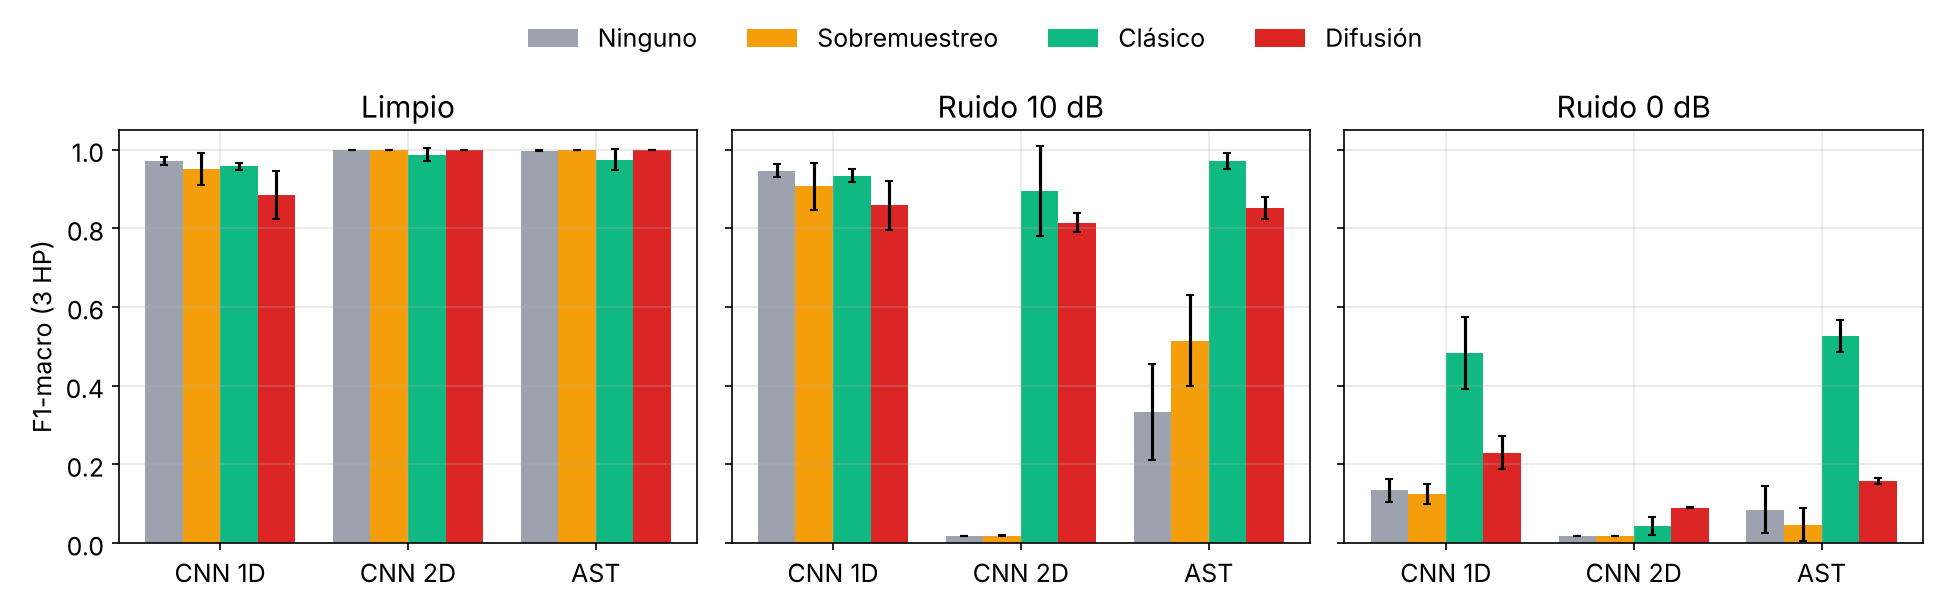
\includegraphics[width=0.92\textwidth]{figs/f1_ruido.png}
\begin{columns}[T]
\column{0.32\textwidth}\small
\textbf{Limpio:} CNN 2D y AST llegan a \num{1,000}; la línea base, a \num{0,972}. El cambio de carga queda casi resuelto.
\column{0.32\textwidth}\small
\textbf{10~dB:} sin aumento, la CNN 2D \alert{colapsa} (0,018) y el AST cae a 0,333.
\column{0.32\textwidth}\small
\textbf{0~dB:} solo el aumento \textbf{clásico} resiste (AST 0,527; CNN 1D 0,484).
\end{columns}
\end{frame}

\begin{frame}{Ablación: ¿difusión o solo equilibrar clases?}
\begin{columns}[c]
\column{0.55\textwidth}
\centering
\begin{tabular}{lccc}
\toprule
F1 a 10~dB & Ninguno & Sobremuestreo & \textbf{Difusión} \\ \midrule
CNN 2D & 0,018 & 0,019 & \num{0,815} \\
AST & 0,333 & 0,514 & \num{0,851} \\
\bottomrule
\end{tabular}
\vspace{4mm}
\small Mismo número de ventanas por clase en sobremuestreo y difusión.
\column{0.42\textwidth}
\begin{exampleblock}{Conclusión}
La mejora viene del \textbf{contenido} de las muestras generadas, no del equilibrio de clases.
\end{exampleblock}
\small Explicación plausible: las sintéticas conservan un piso de ruido de banda ancha que actúa como \alert{aumento de ruido implícito}.
\end{columns}
\end{frame}

\begin{frame}{Calidad de las muestras sintéticas}
\begin{columns}[T]
\column{0.5\textwidth}
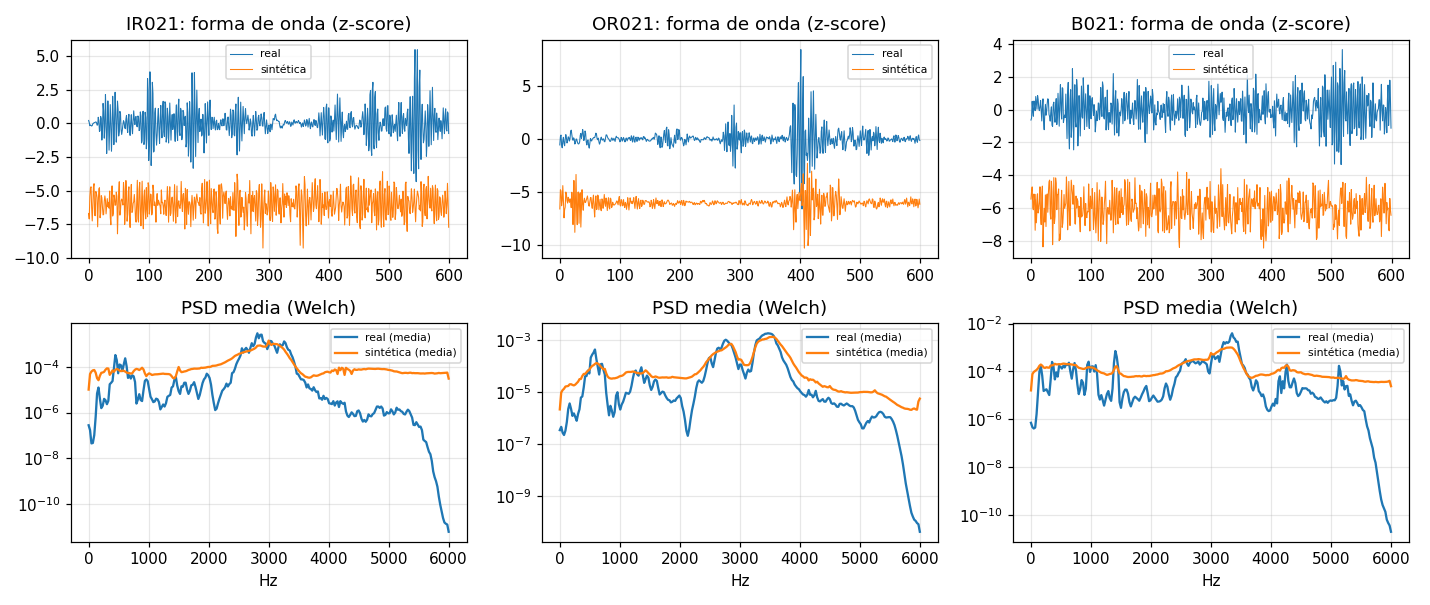
\includegraphics[width=\linewidth]{figs/fig04_real_vs_sintetico.png}\\
\small Reproducen los impactos y la resonancia de 2,5--3,5~kHz; queda ruido en altas frecuencias.
\column{0.48\textwidth}
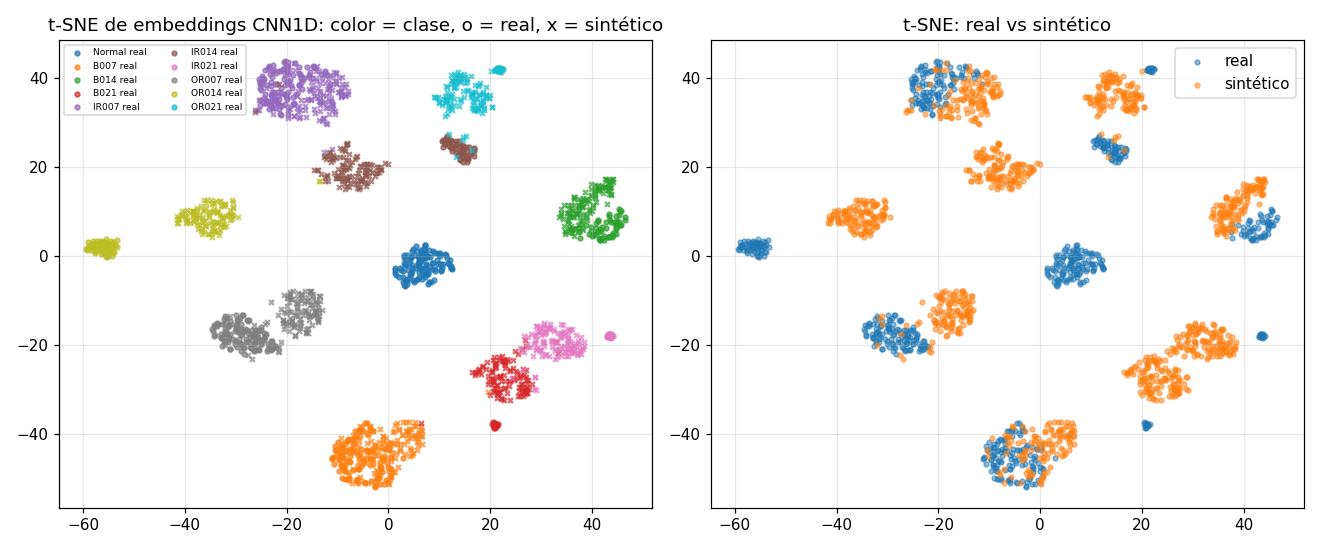
\includegraphics[width=\linewidth]{figs/fig11_tsne.png}\\
\small
\textbf{TSTR} (entrenar solo con sintéticas): F1 = \num{0,680 $\pm$ 0,071}.\\
Pico físico de envolvente correcto: 98--100\,\% en IR007/OR007, \alert{16--20\,\%} en IR014/IR021.
\end{columns}
\end{frame}

% =====================================================================
\section{Interpretabilidad}

\begin{frame}{¿Qué mira la red? Grad-CAM}
\centering
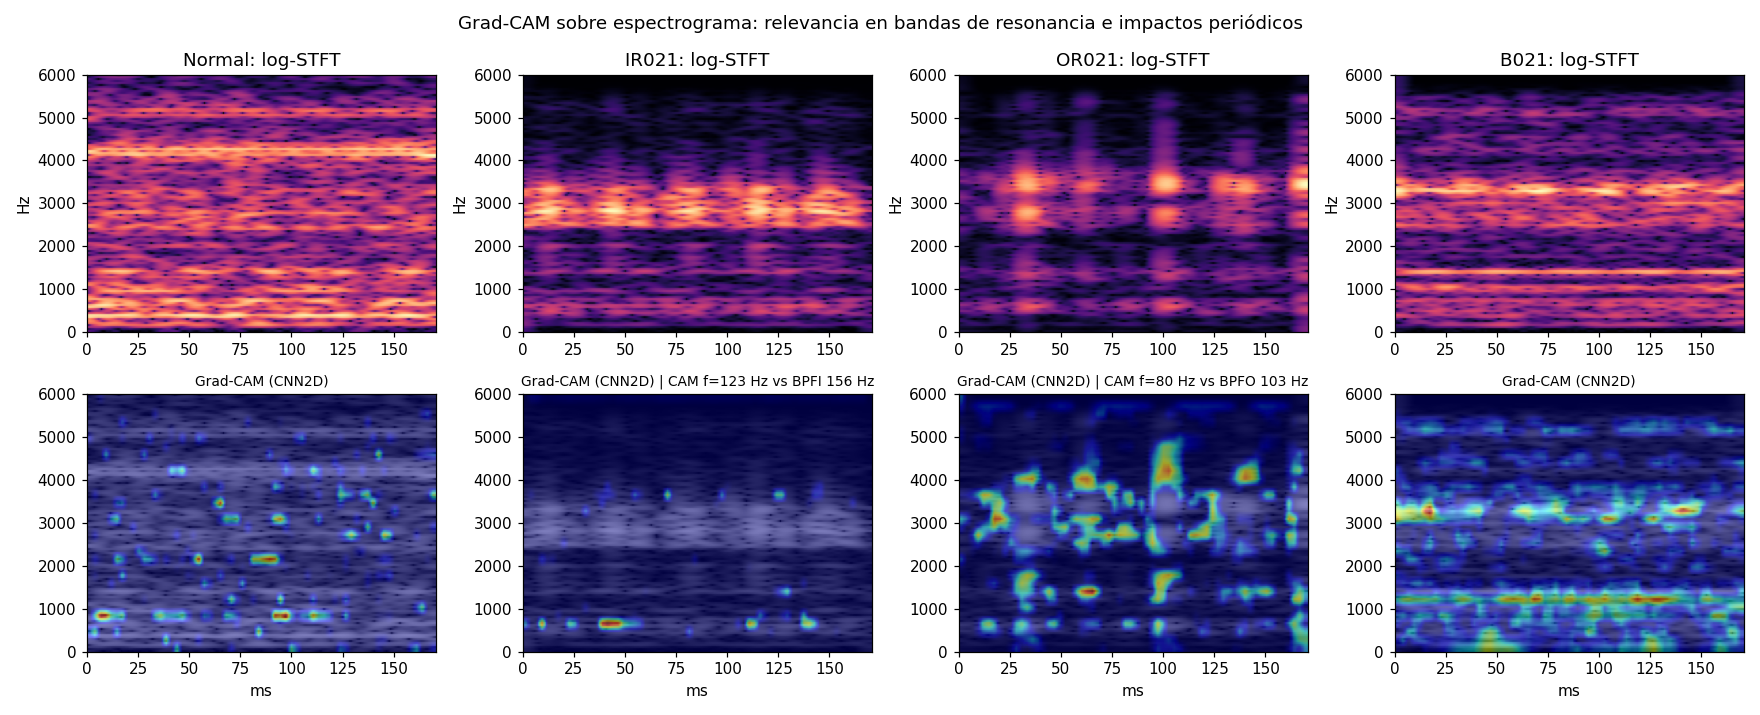
\includegraphics[width=0.82\textwidth]{figs/fig08_gradcam_2d.png}
\begin{columns}[T]
\column{0.5\textwidth}\small
Centroide del Grad-CAM entre \num{2,0 y 3,7~kHz}: la \textbf{banda de resonancia} que excitan los impactos.
\column{0.48\textwidth}\small
Pero la periodicidad del mapa coincide con BPFO/BPFI solo en \alert{0--30\,\%} (la envolvente cruda: 97--100\,\%).
\end{columns}
\end{frame}

% =====================================================================
\section{Discusión y conclusiones}

\begin{frame}{Discusión: limitaciones, sesgos y uso responsable}
\begin{columns}[T]
\column{0.5\textwidth}
\textbf{Limitaciones}
\begin{itemize}\small
\item Cada falla de CWRU es \textbf{un solo rodamiento} en 4 cargas: se generaliza a una carga nueva, no a un rodamiento nuevo.
\item Daños artificiales (electroerosión), no desgaste real.
\item Normal: una sola grabación por carga.
\item El AST se preentrenó con audio, no con vibración.
\end{itemize}
\column{0.47\textwidth}
\textbf{Uso responsable e impacto}
\begin{itemize}\small
\item Validar en cada máquina antes de usar: riesgo de falsas alarmas o fallas no detectadas.
\item Apoyo al técnico (verificar con la envolvente), \alert{no} parada automática.
\item Las sintéticas no reemplazan datos reales de validación.
\item Útil para pymes peruanas con pocos registros de falla.
\end{itemize}
\end{columns}
\end{frame}

\begin{frame}{Conclusiones y trabajo futuro}
\begin{enumerate}
\item Con particiones sin fuga, la dificultad real de CWRU \textbf{no es el cambio de carga} (F1 = 1,000) sino el \alert{ruido} y el desbalance en modelos pequeños.
\item La difusión aporta \textbf{robustez al ruido} que no se explica por el equilibrio de clases (AST: 0,333 $\to$ 0,851 a 10~dB).
\item El aumento clásico sigue siendo la mejor defensa ante ruido severo (0~dB).
\item Los modelos aprenden la \textbf{firma espectral de la resonancia}, no la periodicidad física de los impactos.
\end{enumerate}
\vspace{2mm}
\textbf{Trabajo futuro:} validar en Paderborn y en equipos peruanos · filtrar sintéticas con criterios físicos (BPFO/BPFI) · CNN 1D en microcontrolador · vida útil remanente con PINNs.
\end{frame}

\begin{frame}[standout]
¡Gracias!\\[4mm]
{\normalsize ¿Preguntas?}\\[6mm]
\qrcode[height=2.4cm]{https://github.com/jafcn09/examenfinal_redes_uniingenieria}\\[2mm]
{\scriptsize github.com/jafcn09/examenfinal\_redes\_uniingenieria}
\end{frame}

% =====================================================================
\appendix
\begin{frame}{Respaldo: Contribuciones}
\begin{enumerate}
\item \textbf{Curación de datos exigente} sobre CWRU: partición por carga sin fuga, desbalance de cola larga, evaluación con ruido y \alert{corrección de dos errores del conjunto} (muestreo de la clase Normal y archivo duplicado).
\item \textbf{Combinación de arquitecturas}: un único DDPM condicional 1D genera ventanas de las clases escasas para tres clasificadores (CNN 1D, CNN 2D, AST).
\item \textbf{Evaluación controlada $3\times4$ con 3 semillas}: el \alert{control de sobremuestreo} separa el efecto de equilibrar clases del aporte del generador; interpretabilidad contrastada con la física (BPFO/BPFI).
\end{enumerate}
\vspace{3mm}
\centering\small Toca tres unidades del curso: \textbf{CNN} · \textbf{Transformers} · \textbf{modelos de difusión}
\end{frame}

\begin{frame}{Respaldo: Clases escasas: efecto mixto en la CNN 1D}
\begin{columns}[c]
\column{0.58\textwidth}
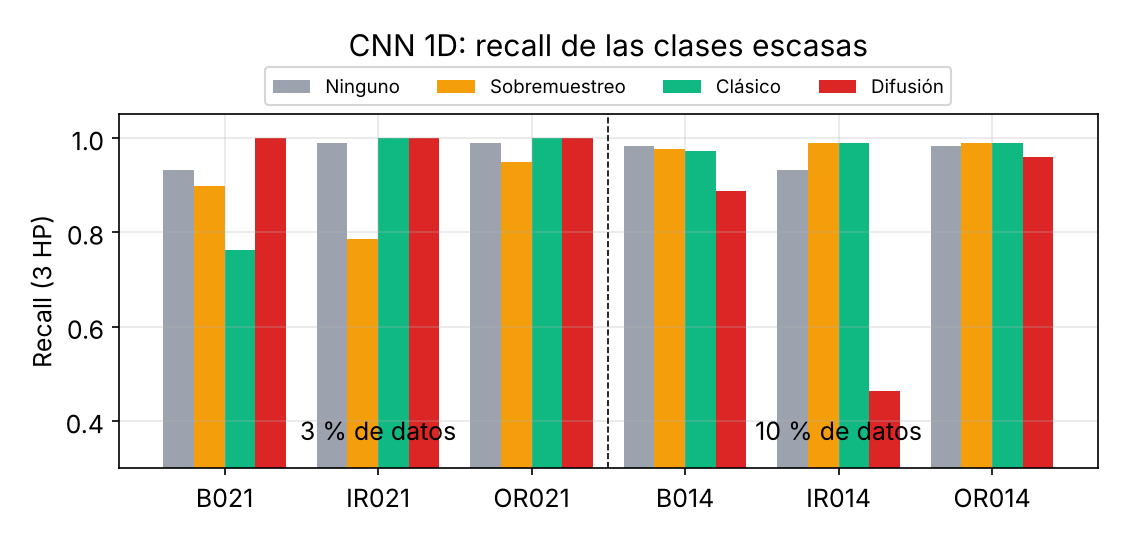
\includegraphics[width=\linewidth]{figs/recall_cnn1d.png}
\column{0.4\textwidth}\small
\begin{itemize}
\item Clases con 3\,\%: recall \num{0,970 $\to$ 1,000} con difusión.
\item Pero IR014 cae a \alert{0,463} $\Rightarrow$ F1 $0{,}885\pm0{,}060$.
\item Sobremuestreo: repetir 16 ventanas \textbf{sobreajusta} (0,878).
\item CNN 2D y AST: $>$0,99 de recall en todas las estrategias.
\end{itemize}
\end{columns}
\end{frame}

\begin{frame}{Respaldo: Análisis de errores}
\centering
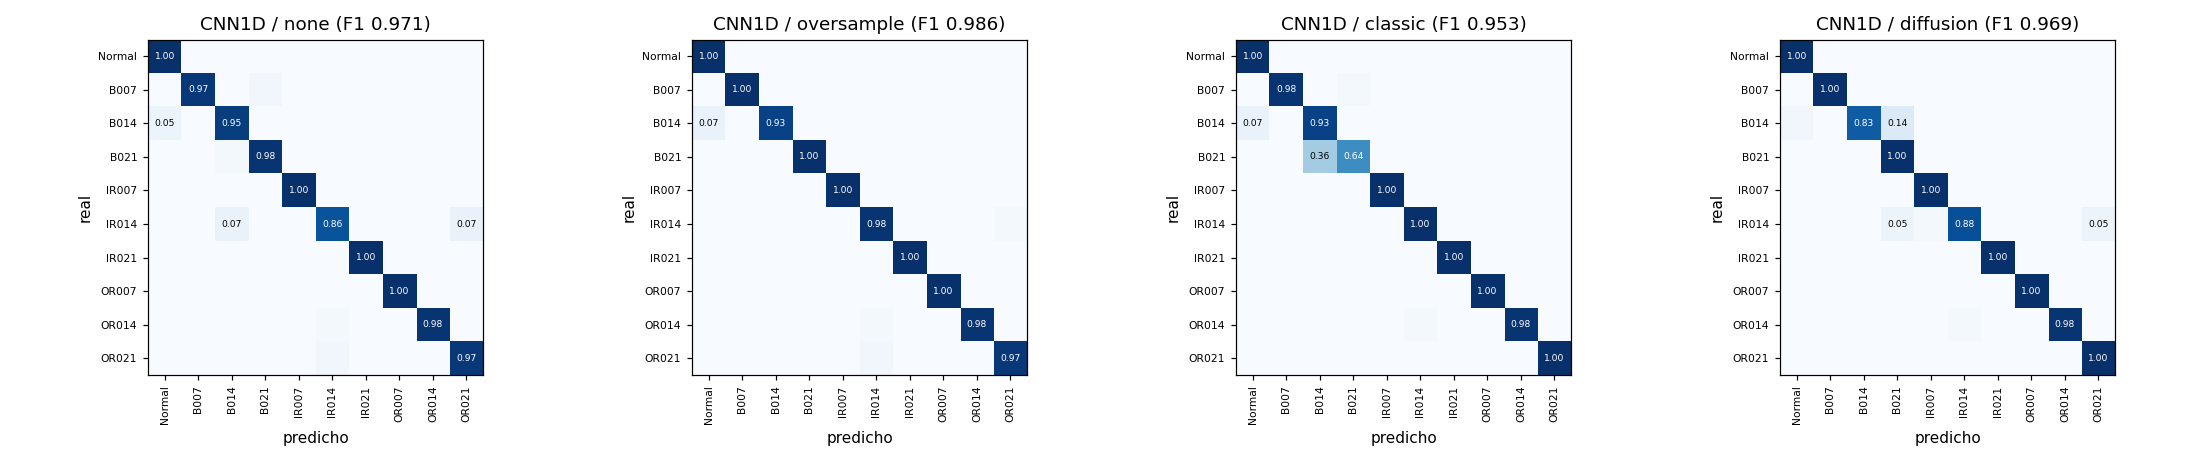
\includegraphics[width=0.95\textwidth]{figs/fig06_matrices_confusion.png}
\begin{itemize}\small
\item En limpio, los errores se concentran en la \textbf{bola} (B014 vs B021) e IR014: las condiciones más difíciles según la envolvente.
\item Con ruido, los modelos sin aumento \alert{predicen todo como Normal}: el ruido de banda ancha se parece al espectro plano del rodamiento sano.
\item La atención del AST es casi uniforme, con un leve máximo en 3,3~kHz para las fallas.
\end{itemize}
\end{frame}

\begin{frame}{Respaldo: Costo computacional}
\begin{columns}[c]
\column{0.48\textwidth}
\centering
\begin{tabular}{lcc}
\toprule
Modelo & Parámetros & ms/ventana (CPU) \\ \midrule
CNN 1D & \num{0,04~M} & \num{0,03} \\
CNN 2D & 0,24~M & 15,8 \\
AST & 85~M & 86,1 \\
\bottomrule
\end{tabular}
\column{0.48\textwidth}
\begin{itemize}\small
\item Todos los experimentos: \num{0,95~h} de GPU (Tesla T4).
\item Las 12 corridas del AST: 63\,\% del tiempo.
\item La CNN 1D tiene \textbf{$\sim$2000 veces menos parámetros} que el AST $\Rightarrow$ candidata para un microcontrolador junto a la máquina.
\end{itemize}
\end{columns}
\end{frame}

\begin{frame}{Respaldo: resultados completos (3~HP, 3 semillas)}
\centering\footnotesize
\begin{tabular}{llcccc}
\toprule
Modelo & Aumento & F1-macro & F1 (10~dB) & F1 (0~dB) & Exactitud \\ \midrule
CNN 1D & Ninguno & 0,972 $\pm$ 0,010 & 0,947 $\pm$ 0,016 & 0,134 $\pm$ 0,028 & 0,972 $\pm$ 0,010 \\
CNN 1D & Sobremuestreo & 0,952 $\pm$ 0,041 & 0,907 $\pm$ 0,061 & 0,125 $\pm$ 0,025 & 0,954 $\pm$ 0,037 \\
CNN 1D & Clásico & 0,958 $\pm$ 0,009 & 0,934 $\pm$ 0,016 & 0,484 $\pm$ 0,091 & 0,959 $\pm$ 0,009 \\
CNN 1D & Difusión & 0,885 $\pm$ 0,060 & 0,859 $\pm$ 0,062 & 0,230 $\pm$ 0,043 & 0,896 $\pm$ 0,052 \\
CNN 2D & Ninguno & 1,000 $\pm$ 0,000 & 0,018 $\pm$ 0,000 & 0,018 $\pm$ 0,000 & 1,000 $\pm$ 0,000 \\
CNN 2D & Sobremuestreo & 1,000 $\pm$ 0,000 & 0,019 $\pm$ 0,001 & 0,018 $\pm$ 0,000 & 1,000 $\pm$ 0,000 \\
CNN 2D & Clásico & 0,988 $\pm$ 0,017 & 0,895 $\pm$ 0,115 & 0,044 $\pm$ 0,024 & 0,988 $\pm$ 0,017 \\
CNN 2D & Difusión & 1,000 $\pm$ 0,000 & 0,815 $\pm$ 0,024 & 0,090 $\pm$ 0,002 & 1,000 $\pm$ 0,000 \\
AST & Ninguno & 0,997 $\pm$ 0,002 & 0,333 $\pm$ 0,122 & 0,086 $\pm$ 0,059 & 0,997 $\pm$ 0,002 \\
AST & Sobremuestreo & 1,000 $\pm$ 0,000 & 0,514 $\pm$ 0,115 & 0,047 $\pm$ 0,041 & 1,000 $\pm$ 0,000 \\
AST & Clásico & 0,975 $\pm$ 0,027 & 0,971 $\pm$ 0,020 & 0,527 $\pm$ 0,040 & 0,977 $\pm$ 0,025 \\
AST & Difusión & 0,999 $\pm$ 0,001 & 0,851 $\pm$ 0,028 & 0,158 $\pm$ 0,007 & 0,999 $\pm$ 0,001 \\
\bottomrule
\end{tabular}
\end{frame}

\begin{frame}{Respaldo: lo que ``ve'' cada modelo}
\centering
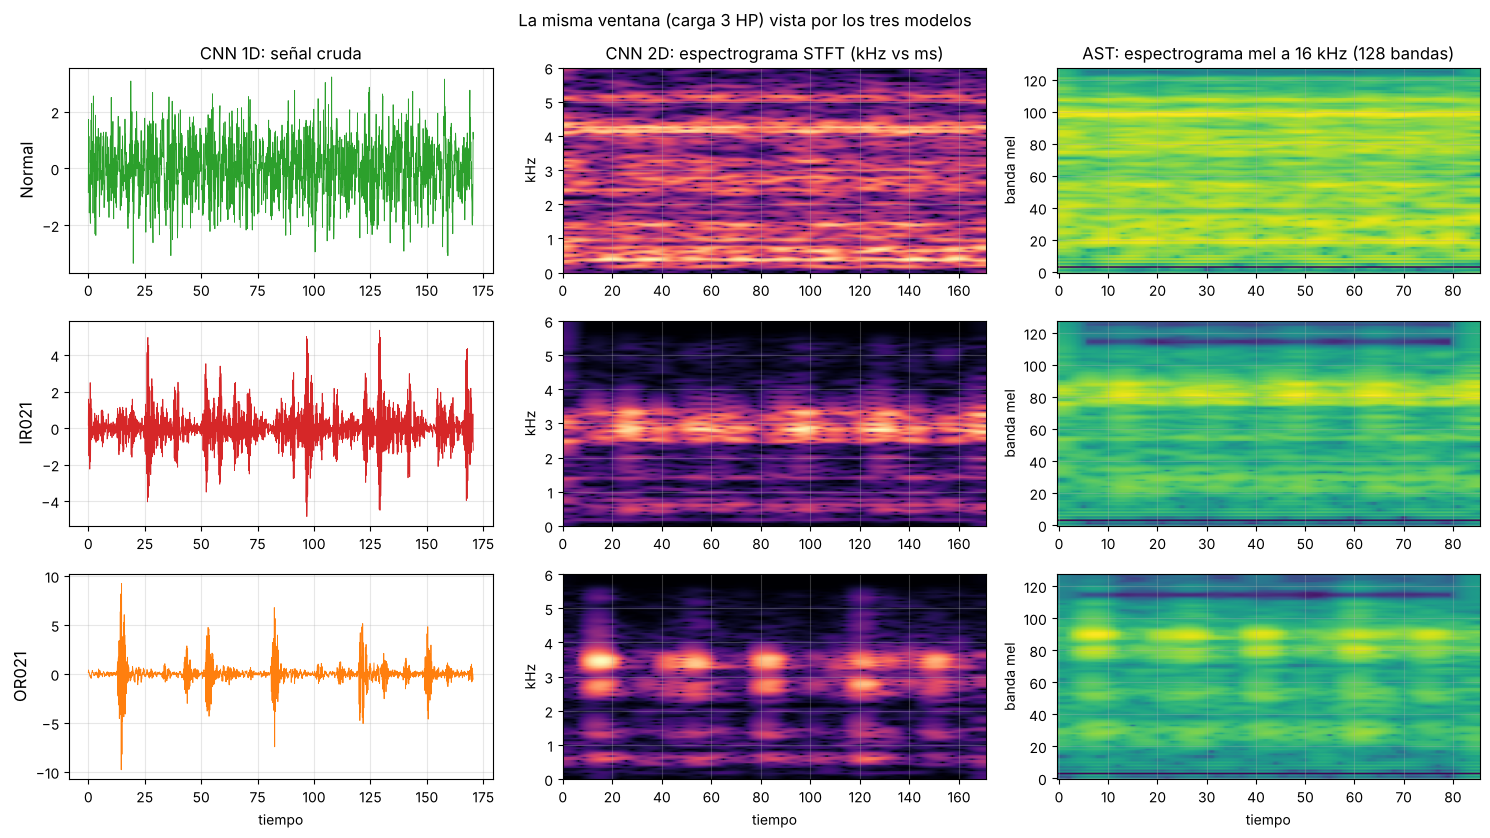
\includegraphics[width=0.75\textwidth]{figs/vistas_modelos.png}\\
\small En las fallas se ven \alert{franjas periódicas}: los impactos repetidos a BPFI / BPFO.
\end{frame}

\begin{frame}{Respaldo: curva del DDPM y Grad-CAM 1D}
\begin{columns}[T]
\column{0.42\textwidth}
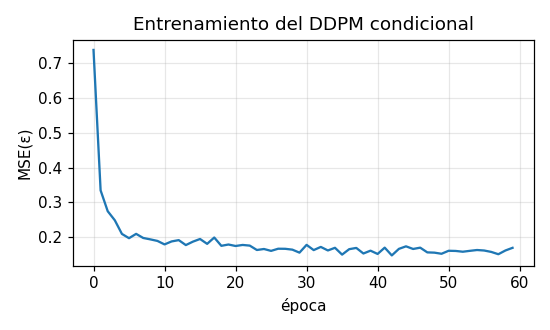
\includegraphics[width=\linewidth]{figs/fig03_difusion_loss.png}
\column{0.56\textwidth}
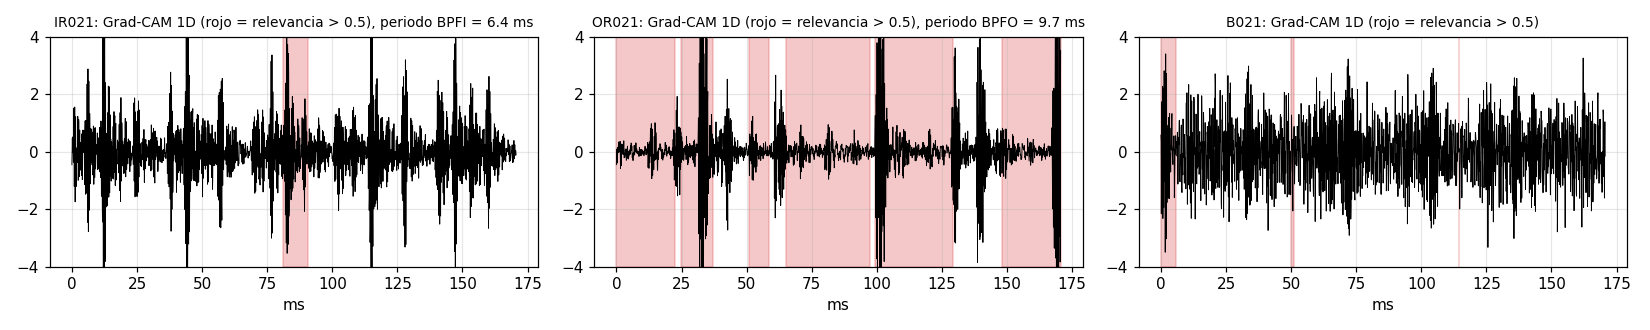
\includegraphics[width=\linewidth]{figs/fig09_gradcam_1d.png}
\end{columns}
\end{frame}

\end{document}
